\documentclass[aspectratio=169]{beamer}

%%%%%%%%%%%%%%%%%%%%%%%%%%%%%%%%%%%%%%%%%%%%%%%%%%%%%%%%%%%%%%%%%%%%%%%%%%%%%%%%%
% PREAMBLE

% DEFINE VARIABLES
\newcommand{\Lesson}{TEMA EJEMPLO}
\newcommand{\Subject}{Ejemplos, ejemplos, y ejemplos}
\newcommand{\Program}{Inversiones Financieras}
\newcommand{\Professor}{CUNEF Universidad}

% FOOTER WITH LOGO
\setbeamertemplate{footline}{
\hfill
\includegraphics[width=1.2cm]{figs/logo.png}\hspace{13cm}\vspace*{0.5cm}
\insertframenumber \hspace{1cm}
}

% FOOTER WITHOUT LOGO
\newcommand{\NoLogoFootline}{
    \setbeamertemplate{footline}{
    \hfill\vspace*{0.5cm}    
    }
}

% IDENTATION OPTIONS
\setlength{\leftmargini}{1em} % for itemize and enumerate level 1
\setlength{\leftmarginii}{1em} % for itemize and enumerate level 2
\setlength{\leftmarginiii}{1em} % for itemize and enumerate level 3

% PACKAGES
\usepackage[absolute,overlay]{textpos}
\usepackage{graphicx, tikz,xcolor}
\usepackage{multirow, bigstrut,epstopdf}
\usepackage{amsmath,relsize,bigdelim}
\usepackage{hyperref}
\hypersetup{
    colorlinks=true,
    linkcolor=blue,
    filecolor=magenta,      
    urlcolor=cyan,
}
\usepackage[font=tiny]{caption}

% COLOR OPTIONS
\definecolor{CUNEFOrange}{RGB}{255, 87, 0}
\definecolor{CUNEFGray}{RGB}{214, 209, 196}
\definecolor{Front}{RGB}{21,31,108}
% BEAMER OPTIONS
\setbeamertemplate{navigation symbols}{}
\setbeamercolor{itemize item}{fg = CUNEFOrange}
\setbeamercolor{itemize subitem}{fg = CUNEFOrange}
\setbeamercolor{itemize subsubitem}{fg = CUNEFOrange}		
\setbeamercolor{enumerate item}{fg = CUNEFOrange}
\setbeamercolor{enumerate subitem}{fg = CUNEFOrange}
\setbeamercolor{enumerate subsubitem}{fg = CUNEFOrange}		
\setbeamercolor{normal text}{fg=Front}

\setbeamercolor{frametitle}{fg=CUNEFOrange}


% NEW TITLE SLIDE
\newcommand{\CUNEFTitleSlide}{\begin{frame}

%\begin{textblock*}{0.1\paperwidth}(0.01\paperwidth,0.01\paperwidth)
%\includegraphics[width=0.3\paperwidth]{Logo_WQU.png}
%\end{textblock*}

\vspace{2em}
%\centering\scriptsize{{\textcolor{CUNEFOrange}{\Lesson}}} \\[1em]
\centering\textbf{{\large\textcolor{CUNEFOrange}{Econometrics 2024/2025}}} \\ [1em]
\centering{\large\textcolor{CUNEFOrange}{}} \\ [1em]
\vspace{0.5em}
\centering{\normalsize\textcolor{CUNEFOrange}{Introduction}}
\end{frame}}

% NEW SLIDE TEMPLATE
\newcommand{\slide}[2]{\begin{frame}
%\begin{textblock*}{0.1\paperwidth}(0.01\paperwidth,0.01\paperwidth)
%\includegraphics[width=0.15\paperwidth]{Logo_WQU.png}
%\end{textblock*}


\begin{textblock*}{0.87\paperwidth}(0.05\paperwidth,1.2cm)
{\Large\textcolor{CUNEFOrange}{#1}}
\end{textblock*}

\begin{textblock*}{0.87\paperwidth}(0.05\paperwidth,2cm)
#2
\end{textblock*}

\begin{textblock*}{\paperwidth}(0.01\paperwidth,0.95\paperheight)
\noindent\begin{tikzpicture}
%\draw[CUNEFOrange] (0,0) rectangle (0.9\paperwidth,0.8em);
%\draw[CUNEFOrange] (0.9\paperwidth+0.01\paperwidth,0) rectangle (\paperwidth-0.02\paperwidth,0.8em);
%\node[right] at (0,0.4em) {\tiny\textcolor{CUNEFGray}{\Subject\enspace-- \Program\enspace-- \Professor\enspace}};
\end{tikzpicture}
{\tiny\textcolor{CUNEFGray}\thepage}
\end{textblock*}
\end{frame}
}
%%%%%%%%%%%%%%%%%%%%%%%%%%%%%%%%%%%%%%%%%%%%%%%%%%%%%%%%%%%%%%%%%%%%%%%%%%%%%%%%%


\begin{document}

%%%%%%%%%%%%%%%%%%%%%
% Title Page
%%%%%%%%%%%%%%%%%%%%
\NoLogoFootline
{\usebackgroundtemplate{%
  
\includegraphics[width=\paperwidth,height=\paperheight]{figs/title_page.png}}
\CUNEFTitleSlide}

%%%%%%%%%%%%%%%%%%%%%
% Organizational issues
%%%%%%%%%%%%%%%%%%%%
\setbeamertemplate{footline}{
\hfill
\includegraphics[width=1.2cm]{figs/logo.png}\hspace{13cm}\vspace*{0.5cm}
\insertframenumber \hspace{1cm}
}

\frame<beamer>{\frametitle{\textcolor{CUNEFOrange}{Organizational issues}}

\begin{itemize}
    \item E-mail: \textbf{andre.santos@cunef.edu}
    \item Office hours: Monday and Wednesday 11:00-13:00, either in person or via Zoom (send an email beforehand!)

    \item Software: The course will use R for all computer-based exercises.
    
    \item Evaluation: 
    \begin{itemize}
\item Continuous evaluation 40\%
\begin{itemize}
\item[-] 30\% Paper-based midterm exam, in-class
\item[-] 10\% R-based group project
\end{itemize}
\item Final exam 60\%
\begin{itemize}
\item[-] Covers all topics 
\item[-] Minimum grade is 5!
    \end{itemize}
\end{itemize}
\end{itemize}
}

\frame<beamer>{\frametitle{\textcolor{CUNEFOrange}{Organizational issues}}

\begin{itemize}

    \item \textbf{Speaking in class}: You can only speak to contribute something to the class or to ask a question. People who disrupt the class will be expelled from the classroom. \medskip

    \item \textbf{Mobile phones}: They must remain in the backpack/bag during the class. \medskip

    \item \textbf{Laptops}: They can be used for taking notes. We will use the laptop for practical class activities.\medskip

    \item \textbf{Punctuality}: You cannot enter the classrooms once the class has started.

\end{itemize}
}


\frame<beamer>{\frametitle{\textcolor{CUNEFOrange}{Organizational issues}}
\centering
\huge\alert{EVERYTHING is in CANVAS}
}

%%%%%%%%%%%%%%%%%%%%%
% Bibliography
%%%%%%%%%%%%%%%%%%%%

\frame<beamer>{\frametitle{\textcolor{CUNEFOrange}{Bibliography}}
\centering

\begin{figure}
    \centering
    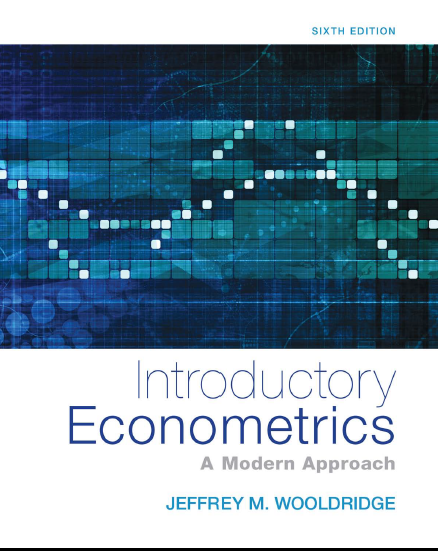
\includegraphics[width=0.4\linewidth]{figs/wooldridge.png}
\caption*{\url{https://encuentra.cunef.edu/permalink/34CUNEF_INST/1k9j0s0/alma991000155609708131}
}
\end{figure}


}


\frame<beamer>{\frametitle{\textcolor{CUNEFOrange}{Bibliography}}
\centering

\begin{figure}
    \centering
    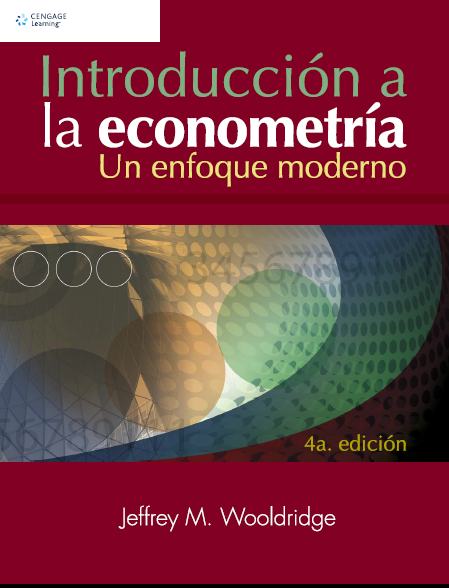
\includegraphics[width=0.4\linewidth]{figs/wooldridge_esp.png}
\caption*{\url{https://encuentra.cunef.edu/permalink/34CUNEF_INST/3hqjvi/alma991000432080008131}
}
\end{figure}


}

\frame<beamer>{\frametitle{\textcolor{CUNEFOrange}{Bibliography}}
\centering

\begin{figure}
    \centering
    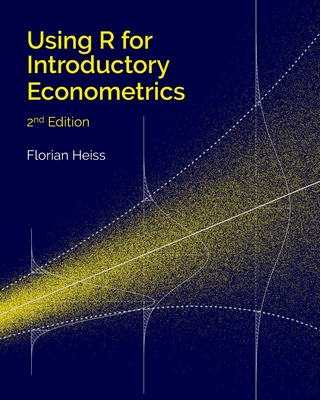
\includegraphics[width=0.4\linewidth]{figs/heiss.png}
\caption*{\url{https://www.urfie.net/downloads/PDF/URfIE_web.pdf}
}
\end{figure}


}

%%%%%%%%%%%%%%%%%%%%%
% Why study econometrics?
%%%%%%%%%%%%%%%%%%%%

\frame<beamer>{\frametitle{}
\centering
\huge\alert{What is Econometrics?}
}

\begin{frame}
    \frametitle{What is Econometrics?}
    \begin{itemize}
        \item Econometrics is the use of statistical methods to analyze economic data (and other types of data).
        \item Econometrics may require a economic theory to be tested. It certainly requires \textbf{data}.
    
    \item Typical objectives of econometric analysis:
\medskip
    \begin{itemize}
        \item Estimation of relationships between economic variables.
        \begin{itemize}
            \item \textbf{When inflation is high, is unemployment also high?}
        \end{itemize}
        \item Testing economic theories and hypotheses.
        \begin{itemize}
            \item \textbf{Do high levels of inflation cause increases in unemployment?}
        \end{itemize}
        \item Evaluating and implementing government and business policies.
        \begin{itemize}
            \item \textbf{How do Spanish firms react when the European Central Bank raises interest rates?}
        \end{itemize}
        \item Prediction / Forecasting.
        \begin{itemize}
            \item \textbf{How high will unemployment and inflation be next year in Spain?}
        \end{itemize}
    \end{itemize}
    \end{itemize}
\end{frame}


\begin{frame}
    \frametitle{Types of Data}
    \begin{itemize}
        \item Cross-sectional data\medskip
        \item Time series data\medskip
        \item Panel or longitudinal data
    \end{itemize}
\end{frame}

\begin{frame}
    \frametitle{Cross-sectional data sets}
    \begin{itemize}
        \item These may include samples of individuals, households, firms, cities, states, countries, or other units of interest at a given point of time or in a given period.

        \item Example: Cross-sectional data set on wages and other characteristics
            \end{itemize}

\begin{figure}
    \centering
    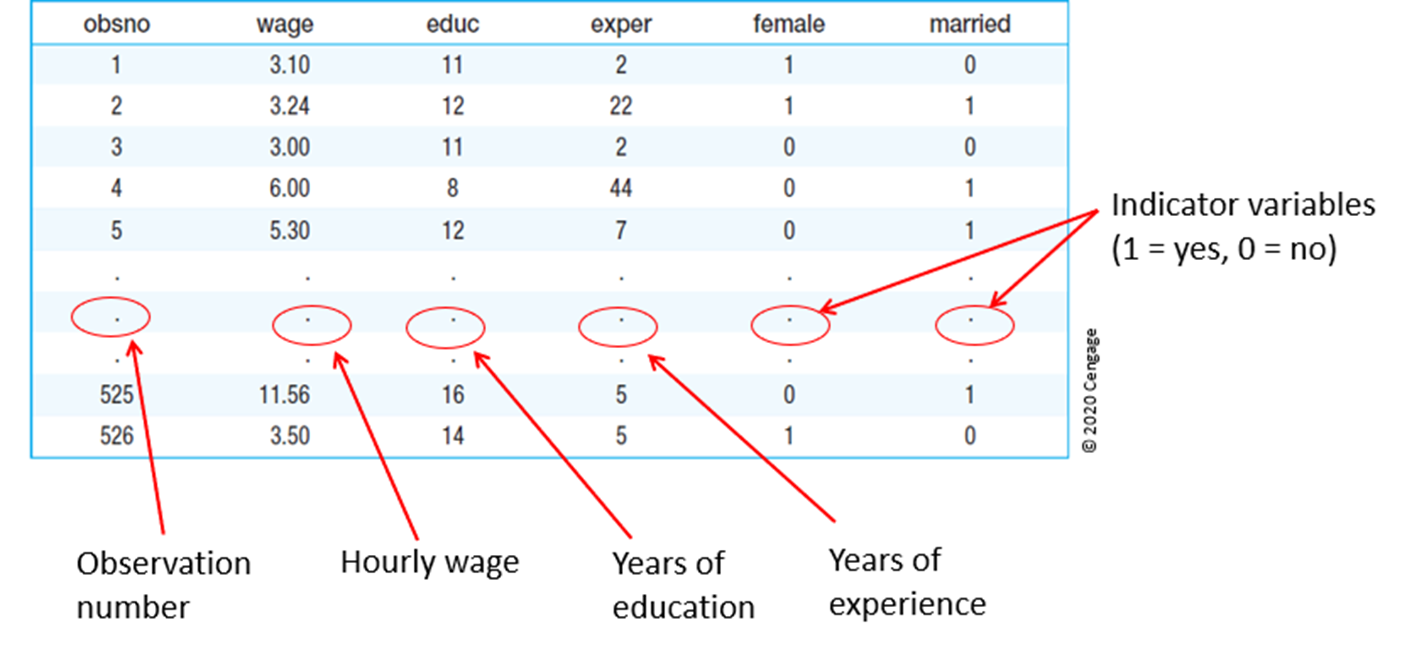
\includegraphics[width=0.8\linewidth]{figs/cross_section.png}
\end{figure}
            
\end{frame}


\begin{frame}
    \frametitle{Time-series data sets}
    \begin{itemize}
        \item This includes observations of a variable or several variables over time.
\item Examples include stock prices, money supply, consumer price index,  gross domestic product, annual homicide rates, automobile sales, and so on.
\item Ordering of observations conveys important information.
\item Data frequency may include daily, weekly, monthly, quarterly, annually, and so on.
            \end{itemize}

\begin{figure}
    \centering
    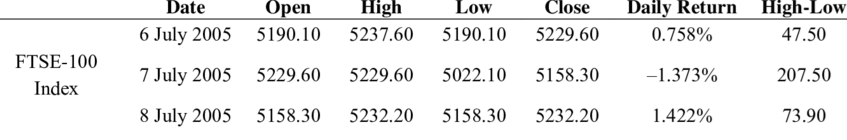
\includegraphics[width=0.8\linewidth]{figs/time_series.png}
\end{figure}
            
\end{frame}


\begin{frame}
    \frametitle{Panel or longitudinal data
 data sets}
    \begin{itemize}
        \item The same cross-sectional units are followed over time.
\item  Panel data have a cross-sectional and a time series dimension.

            \end{itemize}

\begin{figure}
    \centering
    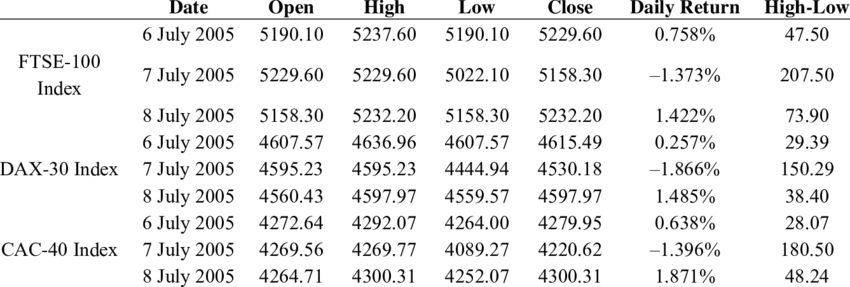
\includegraphics[width=0.8\linewidth]{figs/panel.png}
\end{figure}
            
\end{frame}

%%%%%%%%%%%%%%%%%%%%%
% Back Page
%%%%%%%%%%%%%%%%%%%%
\NoLogoFootline
{\usebackgroundtemplate{%

\includegraphics[width=\paperwidth,height=\paperheight]{figs/back_page.png}}
\slide{}{}}


\end{document}


